\section{Repaso breve de probabilidad}\label{app:probabilidad}

La teoría de probabilidades se basa en postular un espacio
abstracto $\Omega$ en el que se ``sortea'' un elemento $\omega$.
Se asigna una probabilidad $\p{A}\in [0,1]$ a ciertos subconjuntos
$A\subset\Omega$, llamados ``sucesos''.

Si lo aleatorio es un número real, podríamos tomar $\Omega=\R$,
pero en general se piensa en el sorteo como algo que está
``detrás'' y determina el valor $X(\omega)$ a través de una función
$X:\Omega\rightarrow\R$, llamada \emph{variable aleatoria} (V.A.).

\begin{minipage}{0.3\textwidth}La función de distribución de una V.A. se define como $F_X(x)=\p{X\leqslant x}$\end{minipage}\hfill
\begin{minipage}{0.6\textwidth}
    \resizebox{\textwidth}{!}{
    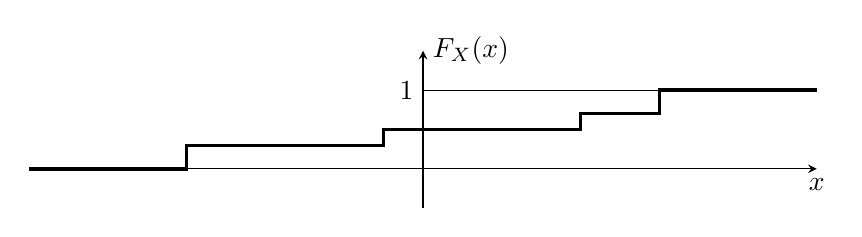
\begin{tikzpicture}
        \draw [-stealth] (-5,0) -- (5,0) node [anchor=north] {$x$};
        \draw [-stealth] (0,-0.5) -- (0,1.5) node [anchor=west] {$F_X(x)$};
        \draw [very thin] (0,1) node [anchor=east] {$1$} -- (5,1);
        \draw [very thick] (-5,0) -- (-3,0) -- (-3,0.3) -- (-0.5,0.3) -- (-0.5,0.5) -- (2,0.5) -- (2,0.7) -- (3,0.7) --  (3,1) -- (5,1);
    \end{tikzpicture}}
\end{minipage}

$F_X(x)$ está entre $0$ y $1$, es monótona no decreciente y continua a
la derecha.

\begin{ejemplo}[Variable aleatoria discreta]
    \begin{minipage}{0.3\textwidth}
        $X$ toma sólo los valores $\{x_1, \ldots, x_N\}$.
    \end{minipage}\hfill
    \begin{minipage}{0.6\textwidth}
    \resizebox{\textwidth}{!}{
    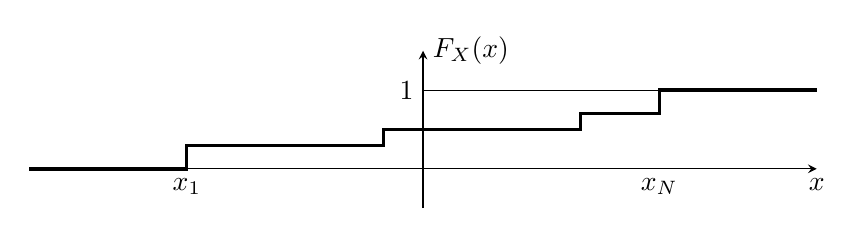
\begin{tikzpicture}
        \draw [-stealth] (-5,0) -- (5,0) node [anchor=north] {$x$};
        \draw [-stealth] (0,-0.5) -- (0,1.5) node [anchor=west] {$F_X(x)$};
        \draw [very thin] (0,1) node [anchor=east] {$1$} -- (5,1);
        \draw [very thick] (-5,0) -- (-3,0) -- (-3,0.3) -- (-0.5,0.3) -- (-0.5,0.5) -- (2,0.5) -- (2,0.7) -- (3,0.7) --  (3,1) -- (5,1);
        \path (-3,0) node [anchor=north] {$x_1$} -- (3,0) node [anchor=north] {$x_N$};
    \end{tikzpicture}}

    Cada salto es $p_i=\p{X=x_i}$.
    \end{minipage}
\end{ejemplo}

\begin{ejemplo}[Variable aleatoria absolutamente continua]
    Existe una densidad $f_X(x)=\frac{\d{}}{\d{} x}F_X(x)$.
    \begin{figure}[htb]
        \hfil
        \begin{tikzpicture}[xscale=0.7]
            \draw [-stealth] (-5,0) -- (5,0) node [anchor=north] {$x$};
            \draw [-stealth] (0,-0.5) -- (0,1.5) node [anchor=west] {$F_X(x)$};
            \draw [dotted] (-5,1) -- (0,1) node [anchor=south east] {$1$} -- (5,1);
            \draw [samples=2000,domain=-4.5:4.5] plot (\x,{rad(atan(\x))/(pi)+0.5});
        \end{tikzpicture}
        \hfill
        \begin{tikzpicture}[xscale=0.7]
            \draw [-stealth] (-5,0) -- (5,0) node [anchor=north] {$x$};
            \draw [-stealth] (0,-0.5) -- (0,1.5) node [anchor=west] {$f_X(x)$};
            \draw [samples=2000,domain=-4.5:4.5] plot (\x,{1/(1+(\x)^2)});
        \end{tikzpicture}
        \hfil
    \end{figure}
    \FloatBarrier

    \[\p{a<X\leqslant b} = F_X(b)-F_X(a) = \int_a^b f_X(x)\d x.\]
\end{ejemplo}

\begin{remark}
Se puede definir una densidad para las V.A. discretas si se
aceptan en ella $\delta$'s de Dirac. Es decir, en este caso \[
 f_X(x)=\sum_i p_i \delta(x-x_i).\]
 Esta convención se adopta en lo que sigue.
\end{remark}

\subsection*{Valor esperado de una variable aleatoria}
\[
\E{X} =\int_{-\infty}^\infty x f_X(x)\d x. \]

Representa el promedio ponderado por la probabilidad. Notar que en
el caso de las V.A. discretas, lo anterior equivale a
$\E{X}=\sum_i x_ip_i$.

\textbf{Momento de orden $k$:}
\[\E{X^k}=\int_{-\infty}^\infty x^kf_X(x)\d x. \]

\textbf{Varianza:} $\var(X)=\E{X^2}-\E{X}^2$.

\begin{ejemplo}[Variable aleatoria Gaussiana]
    \[f_X(x)=\frac{1}{\sqrt{2\pi}\sigma}\e^{-\frac{(x-\mu)^2}{2\sigma^2}}; \quad  \E{X}=\mu, \qquad
    \var(X)=\sigma^2.\]
\end{ejemplo}

Distribución \emph{conjunta} de $n$ variables aleatorias $X_1,
X_2,\ldots, X_n$:

\[F_{X_1,\ldots,X_n}(x_1,x_2,\ldots,x_n)=\p{X_1\leqslant x_1,\ldots, X_n\leqslant x_n}.\]

\subsection*{Probabilidad condicional}

Dados dos sucesos $A,B$ con $\p{B}>0$, la probabilidad de $A$ \emph{condicional} a $B$ es
\[\p{A\mid B} = \frac{\p{A\cap B}}{\p{B}}.\]
Si los sucesos $B_1,\ldots,B_n$ forman una partición de $\Omega$, vale la \emph{fórmula de probabilidad total}:
\[\p{A} = \sum_{i=1}^n \p{A\mid B_i}\p{B_i}.\]
Análogamente, si $A$ es una V.A. discreta que toma valores $a_i$, la \emph{densidad condicional} $f_{Y|A=a_i}(y)$ es la densidad de $Y$ cuando se sabe que ocurrió $\{A=a_i\}$, y se tiene
\[f_Y(y) = \sum_i f_{Y|A=a_i}(y)\,\p{A=a_i}.\]

\subsection*{Independencia}

\begin{itemize}
    \item 2 sucesos $A,B\subset\Omega$ son independientes si $\p{A\cap
    B}=\p{A}\p{B}$.
    \item 2 V.A. $X$, $Y$, son independientes si los sucesos $\{X\leqslant x\}, \{Y\leqslant y\}$
    son independientes para todo $x, y$, es decir
    \begin{align*}
                                           % \underbrace{)} & = P(X\leqslant x)P(Y\leqslant y)\\
                                            F_{XY}(x,y) & = F_X(x)
                                            F_Y(y).
                                        \end{align*}
\end{itemize}

\begin{proposicion}
    Si $X,Y$ son independientes, entonces $\E{XY}=\E{X}\E{Y}$.
\end{proposicion}

Este valor esperado también es una forma de \emph{correlación}. Si
$X(\omega)$ e $Y(\omega)$ se ``acompañan'', $\E{XY}$ da grande.
$\langle X,Y\rangle=\E{XY}$ es un producto interno entre V.A. de
$\E{X^2}$ finito.

La \emph{covarianza} de 2 V.A. se define como
$\E{\left(X-\E{X}\right)\left(Y-\E{Y}\right)}=\E{XY}-\E{X}\E{Y}$.
Si $X,Y$ son independientes, entonces $\mathrm{Cov}(X,Y)=0$. Cuando $\mathrm{Cov}(X,Y)=0$ se dice que las variables están \emph{no correlacionadas}. El recíproco no vale en general, aunque sí para variables \emph{conjuntamente} Gaussianas, como veremos a continuación.

\subsection*{Vectores Gaussianos}

Un vector aleatorio $(X_1,\ldots,X_n)$ es \emph{conjuntamente Gaussiano} si toda combinación lineal $\sum_i c_i X_i$ es una V.A. Gaussiana. En ese caso su distribución conjunta queda completamente determinada por las medias $\E{X_i}$ y las covarianzas $\mathrm{Cov}(X_i,X_j)$. En particular, si las componentes de un vector conjuntamente Gaussiano son no correlacionadas, entonces son independientes. Notar que no alcanza con que cada $X_i$ sea Gaussiana por separado: existen pares de V.A. Gaussianas no correlacionadas que no son independientes.
